\section{Building} 

To execute a C program we first have to compile the source code into object files. If there are no issues with the compilation stage the object files can then be linked together to create an executable file. The executable file can then be called from a command line and run. The procedure is shown in figure \ref{compile}. 

\begin{figure}[H]
\centerline{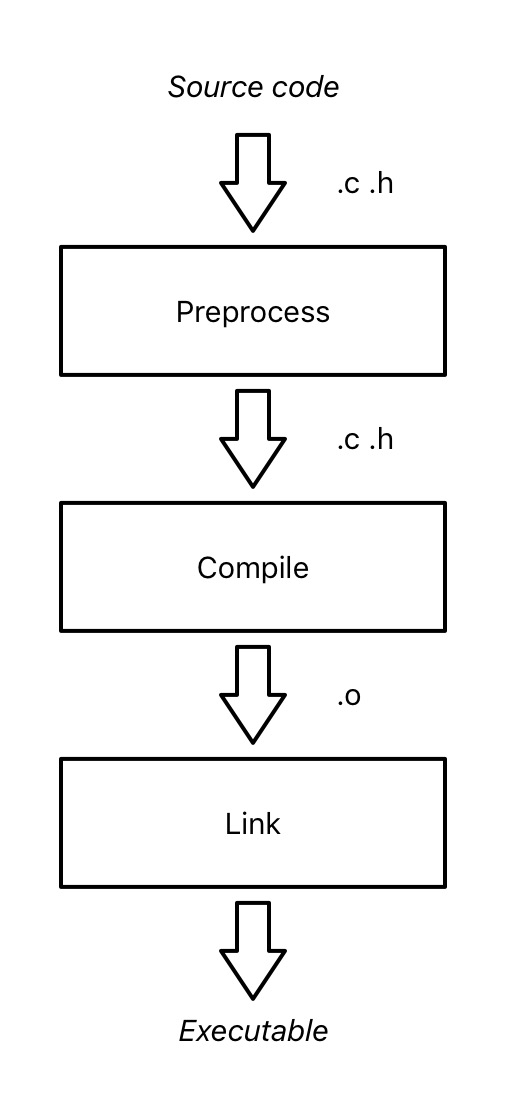
\includegraphics[width=0.3\textwidth]{cycle.jpg}}
\caption{Compile-link process}
\label{compile}
\end{figure}

As already discussed in section \ref{sourcefiles}, a C project is made up of .c and .h files (as well as .s assembler files). When these files are compiled an object or simply a .o file is created. .o files are in a format called ELF (Executable and Linkable Format). The ELF object format is a binary linkable format that cannot be simply read using a standard text editor but can be read by the linker. These types of files are collectively called binary files.

 If there are no errors the .o files can be linked together creating an executable file. The executable file is in what is called an ELF executable format. The ELF executable format contains a standard header at the beginning of the file. This information is used by the Operating System to discover the load address, image type, etc.. The image type defines the hardware architecture that is to be executed. For example, execute type can be AArch64 or x86-64. If an attempt is made to execute on the wrong hardware architecture the Operating System will complain declaring the executable architecture is incompatible.
 
The compiler converts .c and .h files into .o files. For Linux the standard compiler is the GNU C Compiler which is invoked by \textit{cc}, \textit{gcc} or by the more specific full name \textit{arch-elf-gcc}. Note \textit{arch-elf-gcc} is used for cross-compilation, as-in compiling on one architecture to produce binaries for another architecture. For example a typical setup involves developing on a desktop computer and transfer the images to an embedded devices. Cross-compilation is a very common technique with embedded developers. 

\subsection{Compile to executable}

To build the \textit{Hello World} example into an executable, we simply follow the path shown in figure \ref{compile}. This is achieved by compiling the example code \textit{hellow.c} with no options. The compiler will automatically invoke the preprocessor, compiler and finally linker. This will produce an executable image called \textit{a.out}. If the program doesn't include a \textit{main(...)} entry point the linker will throw out an error.\\

\begin{lstlisting}[language=bash,showstringspaces=false,caption={Example compile and execute},captionpos=b,label=simpleb]
 1 $ cc hellow.c
 2 $ ./a.out
 3 Hello World
 4 $ 	
\end{lstlisting}

Listing \ref{simpleb} shows the easiest method to build an executable. Next we want to compile same example but with a specific executable name rather than the generic \textit{a.out}. To achieve this we use the \textit{-o} option.\\ 

\begin{lstlisting}[language=bash,showstringspaces=false,caption={Example compiling and specifying the execution name},captionpos=b,label=hello]
 1 $ cc -o hellow hellow1.c
 2 $ ./hellow
 3 Hello World
 4 $ 	
\end{lstlisting}

Listing \ref{hello} uses the same procedure as the previous example but we build an executable named \textit{hellow} as shown on line:2.

\subsection{Compile to object file}

For larger projects it may be necessary to split the creation of object files and the linking of a final executable. This involves building the object files first before linking them together. This is achieved using the option \textit{-c}. This option instructs the compiler to produce .o files only and not carry out the final linking of an executable image.\\

\begin{lstlisting}[language=bash,showstringspaces=false,caption={Example compiling only, producing object files},captionpos=b,label=linkonly]
 1 $ cc -c hellow1.c
 2 $ ls *.o
 3 hellow.o
 4 $ 	
\end{lstlisting}

Listing \ref{linkonly} shows the link only procedure, with line:1 creating the object file \textit{hellow.o}.

\subsection{Compile with multiple files}

Until now we have exclusively built executables using a single source file but most projects involve multiple files. To build an executable from two or more files we have a slightly different procedure. Listing \ref{multibuild} takes \textit{hellow2.c} and \textit{add.c} respectively and compiles them together, as shown on line:1. Directly creating \textit{a.out} executable file.\\

\begin{lstlisting}[language=bash,showstringspaces=false,caption={Example compiling and linking multiple files},captionpos=b,label=multibuild]
 1 $ cc hellow2.c add.c
 2 $ ./a.out
 3 Hello World, number returned is 2
 4 $ 	
\end{lstlisting}

The next example in listing \ref{multibuild2} takes a mixture of .c and .o files to build an executable. Line:1 shows the \textit{add.o} being created. Line:2 shows \textit{hellow2.c} file being compiled with the previously formed \textit{add.o} file to create an executable called \textit{hello2}.\\

\begin{lstlisting}[language=bash,showstringspaces=false,caption={Example compiling and linking multiple files with a specified execution name},captionpos=b,label=multibuild2]
 1 $ cc -c add.c
 2 $ cc -o hello2 hellow2.c add.o
 3 $ ./hello2 
 4 Hello World, number returned is 2
 5 $ 	
\end{lstlisting}

Line:4 shows the result of adding 1 and 1 together and outputting the result to the console.

\subsection{Libraries}

\index{building libraries}
\index{library}

A library is a grouping of related function calls placed into a single file. There are two types of libraries, namely \textit{shared} and \textit{static}. We will leave the shared library for further exploration since this is more Operating System specific. The static library will be explained in more detail here. A static library is a file containing one or more object files. As already described, an object file contains a set of compiled function calls. A library can then be linked to a image to form an executable. They are useful when the same functionality is required by multiple programs.\\  

\begin{lstlisting}[language=bash,showstringspaces=false,caption={File hellow3.c, build library},captionpos=b,label=library]
 1  $ cc -c add.c sub.c
 2  $ ar cvq simple_lib.a add.o sub.o
 3  q - add.o
 4  q - sub.o
 5  $ cc hello3.c simple_lib.a
 6  $ ./a.out
 7  a+b=30
 8  a-b=10 	
\end{lstlisting}

Listing \ref{library} shows how to build a simple library. Line:2 uses the \textit{ar} util tool (also known as the archive tool) to create the library \textit{simple\_lib.a}. This library can then be used to create an executable, as shown on line:5. 

\subsection{Makefile}

\index{makefile}

Make is a powerful build tool. It is used to build larger projects. There are a number of \textit{make} like alternatives that are worth exploring but \textit{make} is useful since it checks for dependencies which allows for incremental builds.

An incremental build is one where only the source files that are newer than the executable are re-compiled. This means not all of the files are re-compiled each time we want to create an executable. This saves a lot of time when dealing with larger projects.\\

\begin{lstlisting}[language=bash,showstringspaces=false,caption={File Makefile, build a program called hello},captionpos=b,label=makefile]
 1 hello : hellow2.o add.o 
 2 		cc -o hello hellow2.o add.o
 3
 4 hellow2.o : hellow2.c add.h
 5  	cc -c hellow2.c
 6 
 7 add.o : add.c add.h 
 8 		cc -c add.c
 9
10 clean :
11 		rm hello hellow2.o add.o

INTERACTION

12 $ make clean
13 rm hello hellow2.o add.o
14 $ make
15 cc -c helloworld2.c
16 cc -c add.c
17 cc -o hello hellow2.o add.o
18 $ ./hello
19 Hello World, number returned is 2
20 $ nano add.c  
21 $ make
22 cc -c add.c
23 cc -o hello hellow2.o add.o
24 $ 
\end{lstlisting}
   
Listing \ref{makefile} shows a simple \textit{make} project. The project builds an executable called \textit{hello} line:1. The dependencies for \textit{hello} are \textit{hellow2.o} and \textit{add.o} respectively. Line:2 shows the final command to build \textit{hello}. The makefile itself is called \textit{Makefile} in the filing system. It can have other names but by default the \textit{make} util looks for that file name unless otherwise directed.

Lines:4:7 shows the dependencies for building specific object files. Lines:5:8 show the compiler command to build the object files. Line:2 is the finished project compiler command to build the executable. Finally line:1 are the dependencies for the executable.


Lines:10:11 specify the \textit{clean} option when \textit{make clean} is typed in on the console. Line:11 removes all the old object files and the current executable leaving just source code.

We have now covered the different aspects of compiling, from a simple compilation of one file to building of a Makefile for more complex projects. Other areas worth exploring, compiling for debug and compiling with assembly files.



    